\pend \newpage [p.~71]
\begin{center}
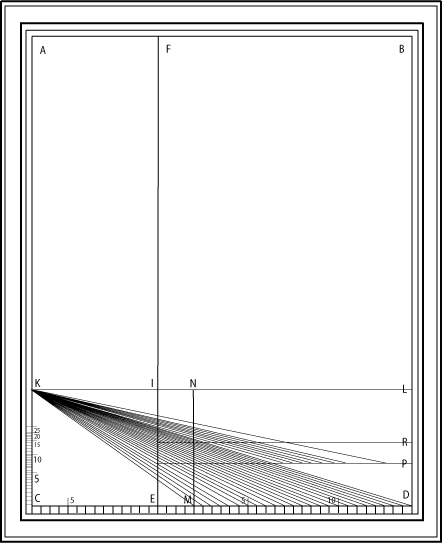
\includegraphics[width=0.75\textwidth]{images/Aleaume_71}
\\\rule[-4mm]{0mm}{10mm}\textit{[Fig. 1]}\footnote{\textit{Neben der Zeichnung rechts unten}: sit \textit{KC c CM m  MD x  MQ y} (fingendo \textit{KQD} esse rectam) fiet \textit{c}:\textit{M} + \textit{x} :: \textit{y}:\textit{x} ergo \textit{y} aeq. \textit{cx}:\textit{M} + \textit{x}. Si ponatur \textit{c} et \textit{M} aequales erit \textit{y} dimidium mediae harmonicae inter \textit{c} et \textit{x}.}
\end{center}
\pstart
\newpage